\documentclass[10pt]{article}


%

\def\Type{LessonCaelan}
\newcommand\TypeNum{Lesson 2}
\newcommand\TypeTitle{Introduction to Limits\\Notes to Instructor }
\newcommand\Semester{Fall 2021} %Not Used 
\newcommand\Course{MATH 1190 \& 1210}
\newcommand\Targets{{\bf\color{RoyalBlue}L1}}
\def\desmosClassCode{{\bf ZAJ$3$AZ}}

\usepackage{preambleDJ}



%%%%%%%%%%%% BEGIN DOCUMENT %%%%%%%%%%%%%%%
%%%%%%%%%%%% BEGIN DOCUMENT %%%%%%%%%%%%%%%
%%%%%%%%%%%% BEGIN DOCUMENT %%%%%%%%%%%%%%%
%%%%%%%%%%%% BEGIN DOCUMENT %%%%%%%%%%%%%%%
%%%%%%%%%%%% BEGIN DOCUMENT %%%%%%%%%%%%%%%

\begin{document}

\pagestyle{otherpages}
%\thispagestyle{empty}
\thispagestyle{firstpage}
%\Heading{MATH 1190 \& 1210 Survey of Calculus I}{\begin{minipage}{0.25\textwidth}\begin{center} Lesson 2:\\ Introduction to Limits \end{center}\end{minipage}}
%
%\vspace{0.1in}
%
%\Name{} \quad \Target{{\bf\color{RoyalBlue}L1}}
%
%\hrulefill

\vs{.75}

\lt  
\enum{
\item[L1:] Limits from tables and graphs
\itemC{
 \item Evaluate both one-sided and two-sided limits of a function based on its graph or on a table of values.
\item Decide when a limit ``$=\infty$" or ``$=-\infty$" using a graph or a table of values.\item Identify the form of a limit in which the independent variable approaches $=\infty$ or $=-\infty$.
}
}

\lg Students will be able to...
\enumCN{
\item  Use a table of data or a graph to infer limits as $x$ approaches $a$ from left/right.
\item Use a table of data or a graph to infer limit as $x$ approaches $a$ and the connection to inferring limits as $x$ approaches $a$ from left/right.
\item Explain  mathematical notation $\ds \lim_{x\to a^{-}} f(x)$, $\ds \lim_{x\to a^{+}} f(x)$ and $\ds \lim_{x\to a} f(x)$ with informal language.
\item Explain the difference between $\ds \lim{x\to a}f(x)$ and $f(a)$.
}

\feed  Please look at student responses to reflection question in Microsoft Forms: ``Is there anything in the pre-class assignment that wasn't clear or that you didn't understand? Was there anything you found especially interesting?" Displaying a sample of these responses a) lets students know you care about what they are doing b) adds some social motivation to keep doing the pre-class activities. 
\itemC{
\item Navigate to Microsoft Forms (see link from Caelan)
\item In upper left corner click on ``Responses"
\item Download copy in Excel
\item Down arrow above column G allows you to sort to see only your section(s).
}
{\em Specific feedback:}
\itemC{
\item Several students thought that the applications of limits were interesting.  
\item Some students wanted more explicit rules/principles for finding limits.  {\em Note to Instructor} These principles/rules are exactly what we are going to elucidate in Exercises A-C. Please tell students we are going to address their concerns!
\item Some students had questions about the 'slow down' example (I think this is GPS example).
\item Some asked questions about why smaller time intervals would be more accurate and wondered about reasoning behind last question on slide 7.
\item Some students needed a reminder about Slide 8 (Summary slide) to click blue icon (blue circle with white ``i") for more information.
}

 \hand
 \itemI{
 \item Warmup Exercise (not on handout) If you did not have enough time to work through details of Exercise C at end of Lesson 1, the Desmos activity {\em AROC vs IROC} might be helpful.. There are two ways you can access the activity.
 \itemI{
  \item \href{https://classroom.amplify.com/activity/66d273076b98f367ec65ead7?utm_campaign=share&utm_content=activity}{Desmos activity {\em AROC vs IROC}}. You can use this in preview mode to demonstrate what's going on.
 \item \url{https://student.desmos.com} (entry code: \desmosClassCode). This version will allow students to use this activity.    Ask students to sign in with UVA email if you want to track responses.
 } If you have a Desmos account feel free to copy and improve this activity.
 \item There are $3$ pairs of Discussion Examples (i.e. interactive examples) and Exercises designed to lead students informally to {\em discover} a more formal statement about a limit. Limit notation is intentionally avoided during the first pass through these exercises, but we'll come back to it later. The Interactive Example of each pair allows the instructor to work with class to discover the trend of $f(x)$ as $x$ approaches $a$ from right and left and concludes with question ``x approaches $a$?"  The Exercise portion of the pair is designed for students to work together and apply the principle just discovered.  
 \item Starting with {\bf Limit of a Function} definition, we begin to introduce more formal notation based on what students saw in pre-class video, This is  followed by a Poll Everywhere (or DJ's  fill-in the blank exercise) to help students connect informal language from first part of handout to more formal limit notation. This exercise can also be implemented as a matching exercise without use of technology.
 \item After the matching/PollEv/Fill-in-blank, cycle back to ``Notation" columns in exercises A-C
 \item Exercise D provides a graph and asks students similar questions as Exercises A-C but using limit notation.  Note that the data on tables was generated by the functions graphed in this example.  
 \item Exam Practice 1 is optional and provides more practice connecting various limits with graphs.
 }

\core Interactive Discussion Examples $1-3$. Exercises A-C, Exercise D.


\newpage
\textbf{Intended Learning Outcomes}
After this lesson, you will be able to 

\begin{itemize}
    \item Describe the meaning of a limit. (\target{L1})
    \item Evaluate both one-sided and two-sided limits of a function based on its graph or on a table of values and vice versa. (\target{L1})
    \item Evaluate two-sided limits by evaluating the respective one-sided limits. (\target{L1})
    \item Decide when a limit “$=\infty$” or “$=-\infty$” and interpret its meaning of such infinite limits.using a graph or a table of values. (\target{L1})
\end{itemize}

\vspace{-0.5cm}

\hrulefill

\vspace{0.3cm}

Problems are solved in calculus by finding ever better approximations of a desired, unknown quantity. The goal of this activity is for us to devise a mathematical tool that will empower us to improve many important approximations - ultimately, making them as accurate as needed - and to use this tool flexibly when given tables and graphs.\\

Let's use the next $3$ exercises to decide upon some properties of such a tool before defining it.\\

%%%%%%%%%%%%%%%%%%%%%%%%

 \ie{\color{RoyalBlue}L1}The table below shows some output values of a function $f$ for input values of $x$ near $0$. 
\nti{
\itemC{
\item Note that  $x=0$ and $f(0)$ do not appear in the table as we want to help students interact with idea that a limit is examination of the trend of the values of $f(x)$ as we approach $x=0$ and not what happens when $x=0$.  
\item I'm planning on  soliciting feedback from whole class here. When we get to last bullet, I probably will ask prompt with "How is this question different from previous two?"  "How might we connect what we did in previous two bullets with this question?" and eventually get to the place where students recognize that trend from both sides must agree in order to conclude answer is $2$ here. 
\item I'm not going to deal with ``Notation" column now but will cycle back after we talk about more formal definition of limit right before Exercise D.
}
}
\begin{center}
\begin{tabular}{| c || c c c c c c |}
\hline
 $x$  & $-0.1$ & $-0.01$ & $-0.001$ &  $0.001$ & $0.01$ & $0.1$\\ 
 \hline
 $f(x)$ & $1.889$ & $1.989$  & $1.999$ & $1.999$   & $1.99$  & $1.9$\\
 \hline
\end{tabular}
\end{center}

\mpageT{.725}{.4}{
Which real value (if any) does $f(x)$ appear to approach as... 
\begin{itemize}
\item $x$ approaches $0$ through values strictly less than $0$?$\dotfill$ \unline{.5}{\blue{$2$}}\\
\item $x$ approaches $0$ through values strictly greater than $0$?$\dotfill$ \unline{.5}{\blue{$2$}} \hs{-.13} \\
\item $x$ approaches $0$?$\dotfill$ \unline{.5}{\blue{$2$}}\\
\end{itemize}
}{
\centering \underline{Notation:}
\blue{$$\lim_{x\to0^-}f(x)=2$$\vs{.025}
$$\lim_{x\to0^+}f(x)=2$$\vs{.025}
$$\lim_{x\to0}f(x)=2$$
}
}
~\\In the space below, write some rules the mathematical tool we're developing should follow based on how we made decisions in this example.

\blue{
Informally:  For $f(x)$ to approach a value (say $2$) as $x$ approaches the target (e.g. $0$), the value of $f(x)$ must be same as $x$ approaches from the left as it is when it approaches from the right. \\\\
More formally using notation developed right before Exercise D: $$\lim_{x\to0} f(x)=2 \text{ if and only if} \lim_{x\to0-} f(x)= \lim_{x\to0+} f(x)=2$$ 
}

\exercise{\color{RoyalBlue}L1} The table from the previous problem has been updated below to include the value of $f(x)$ when $x=0$.
\nti{
\itemC{
\item I"m having students work in pairs or groups.
\item This table now includes $x=0$ and $f(0)=3$
\item Students may need some prompting about fact that $f(0)=3$ is not relevant
}
}
\begin{center}
\begin{tabular}{| c || c c c c c c c |}
\hline
 $x$  & $-0.1$ & $-0.01$ & $-0.001$ & $0$ & $0.001$ & $0.01$ & $0.1$\\ 
 \hline
 $f(x)$ & $1.889$ & $1.989$  & $1.999$ & $3$ & $1.999$   & $1.99$  & $1.9$\\
 \hline
\end{tabular}
\end{center}

\mpageT{.725}{.4}{
Based on the updated table, which real value (if any) does $f(x)$ appear to approach as... 
\begin{itemize}
\item $x$ approaches $0$ through values strictly less than $0$?$\dotfill$ \unline{.5}{\blue{$2$} }\\
\item $x$ approaches $0$ through values strictly greater than $0$?$\dotfill$ \unline{.5}{\blue{$2$}} \hs{-.13} \\
\item $x$ approaches $0$?$\dotfill$ \unline{.5}{\blue{$2$}}\\
\end{itemize}
}{
\centering \underline{Notation:}\\
\blue{$$\lim_{x\to0^-}f(x)=2$$\vs{.025}
$$\lim_{x\to0^+}f(x)=2$$\vs{.025}
$$\lim_{x\to0}f(x)=2$$
}
}

In the space below, write some rules the mathematical tool we're developing should follow based on how we made decisions in this example. You don't have to rewrite any rules established in an earlier problem.

\blue{
Informally:  Same as Interactive Example $1$.  What's new is that   $f(x)$ when $x$ is exactly at target $0$ (i.e. $f(0=3$) has no impact. \\\\
More formally using notation developed right before Exercise D: $$\lim_{x\to0} f(x)=2 \text{ if and only if} \lim_{x\to0-} f(x)= \lim_{x\to0+} f(x)=2$$ 
$f(0)=3$ is irrelevant.
}



\ie{\color{RoyalBlue}L1}The table below shows some output values of the function $f$ for input values of $x$ near $2$. 
\nti{
\itemC{
\item This problem introduces example  of Does Not Exist $=$ DNE.
\item DJ is hoping need for instructor comments decreases after first two examples. It may be the case that students can handle this in groups/pairs with some prompting.  You will want to pay attention to pacing as we have 6 Examples/Exercises to get through.
}
}
\begin{center}
\begin{tabular}{| c || c c c c c c |}
\hline
 $x$  & $1.9$ & $1.99$ & $1.999$ & $2.001$ & $2.01$ & $2.1$\\ 
 \hline
 $g(x)$ & $0.1$ & $0.01$  & $0.001$ & $1.002$   & $1.029$  & $1.271$\\
 \hline
\end{tabular}
\end{center}

\mpageT{.725}{.4}{
Which real value (if any) does $f(x)$ appear to approach as... 
\begin{itemize}
\item $x$ approaches $2$ through values strictly less than $0$?$\dotfill$ \unline{.5}{\blue{$0$} }\\
\item $x$ approaches $2$ through values strictly greater than $0$?$\dotfill$ \unline{.5}{\blue{$1$}} \hs{-.13} \\
\item $x$ approaches $2$?$\dotfill$ \unline{.5}{\blue{Does Not Exist}}\\
\end{itemize}
}{
\centering \underline{Notation:}
\blue{$$\lim_{x\to2^-}f(x)=0$$\vs{.025}
$$\lim_{x\to2^+}f(x)=1$$\vs{.025}
$$\lim_{x\to2}f(x)=DNE$$
}
}


In the space below, write some rules the mathematical tool we're developing should follow based on how we made decisions in this example. You don't have to rewrite any rules established in an earlier problem.

\blue{Informally: When $f(x)$ approaches different values when $x$ approaches target from left compared to from right, we say the limit is DNE or ``Does Not Exist"\\
\\
More formally: 
$$\text{If }\lim_{x\to 2^-}f(x) \neq \lim_{x\to 2^+}f(x) \text{ then }\lim_{x\to 2} f(x) = DNE$$
}

\newpage
\exercise{\color{RoyalBlue}L1} The table from the previous problem has been updated below to include the value of $f(x)$ when $x=2$.

\begin{center}
\begin{tabular}{| c || c c c c c c c |}
\hline
 $x$  & $1.9$ & $1.99$ & $1.999$ & $2$ & $2.001$ & $2.01$ & $2.1$\\ 
 \hline
 $g(x)$ & $0.1$ & $0.01$  & $0.001$ & $0$ & $1.002$   & $1.029$  & $1.271$\\
 \hline
\end{tabular}
\end{center}

\mpageT{.725}{.4}{
Based on the updated table, which real value (if any) does $f(x)$ appear to approach as... 
\begin{itemize}
\item $x$ approaches $2$ through values strictly less than $0$?$\dotfill$ \unline{.5}{\blue{$0$}}\\
\item $x$ approaches $2$ through values strictly greater than $0$?$\dotfill$ \unline{.5}{\blue{$1$}} \hs{-.13} \\
\item $x$ approaches $2$?$\dotfill$ \unline{.5}{\blue{Does Not Exist}}\\
\end{itemize}
}{
\centering \underline{Notation:}\\
\blue{$$\lim_{x\to2^-}f(x)=0$$\vs{.025}
$$\lim_{x\to2^+}f(x)=1$$\vs{.025}
$$\lim_{x\to2}f(x)=DNE$$
}
}

In the space below, write some rules the mathematical tool we're developing should follow based on how we made decisions in this example. You don't have to rewrite any rules established in an earlier problem.

\blue{
No new principle/rule here!  We are applying Exercise A and Interactive Example 2.
}

%%%%%%%%%
%\newpage%
%%%%%%%%%

 \ie{\color{RoyalBlue}L1}The table below shows some output values of the function $f$ for input values of $x$ near $4$. 
\nti{
\itemC{
\item Students should assume trend of $f(x)$ continues as $x$ approaches $4$. 
\item This introduces idea that limit DNE because one sided limits approach $\pm$infinity
\item Exercise C is similar examination of one-side limits to infinity. We want students to not only articulate that limit does not exist as $x$ approaches $4$ but also that it DNE because it approaches $\pm$ infinity. Thus we have DNE for different reasons than in Exercise B. 
}
}
\begin{center}
\begin{tabular}{| c || c c c c c c c |}
\hline
 $x$  & $3.9$ & $3.99$ & $3.999$ & $4$ & $4.001$ & $4.01$ & $4.1$\\ 
 \hline
 $f(x)$ & $4.89$ & $198.99$  & $25,147.13$ & $2$ & $-1,000,000$   & $-10,000$  & $-100$\\
 \hline
\end{tabular}
\end{center}
\mpageT{.725}{.4}{
Which real value (if any) does $h(x)$ appear to approach as... 
\begin{itemize}
\item $x$ approaches $4$ through values strictly less than $4$?\dotfill  \unline{.5}{\blue{$\infty \rightarrow$DNE}}{.125} \\
\item $x$ approaches $4$ through values strictly greater than $4$?\dotfill \unline{.5}{\blue{$-\infty \rightarrow$DNE}}{.125} \\
\item appear to approach as $x$ approaches $4$?\dotfill \unline{.5}{\blue{DNE}}{.125} \\
\end{itemize}
}{
\centering \underline{Notation:}
\blue{$$\lim_{x\to4^-}f(x)=\infty= \rightarrow DNE $$\vs{.025}
$$\lim_{x\to4^+}f(x)=-\infty \rightarrow DNE$$\vs{.025}
$$\lim_{x\to4}f(x)=DNE$$
}
}
In the space below, write some rules the mathematical tool we're developing should follow based on how we made decisions in this example. You don't have to rewrite any rules established in an earlier problem.
\sol{
Informal: when $f(x)$ grows without stopping through positive numbers, we say it grows towards infinity. If $f(x)$ grows without bound (i.e. without stopping) through negative numbers, then it approaches negative infinity.
}
\newpage
\exercise{\color{RoyalBlue}L1} The table from the previous problem has been updated below to correct some typos made in the first table.

\begin{center}
\begin{tabular}{| c || c c c c c c c |}
\hline
 $x$  & $3.9$ & $3.99$ & $3.999$ & $4$ & $4.001$ & $4.01$ & $4.1$\\ 
 \hline
 $f(x)$ & $4.89$ & $198.99$  & $25,147.13$ & $2$ & $1,000,000$   & $10,000$  & $100$\\
 \hline
\end{tabular}
\end{center}
\mpageT{.725}{.4}{
Which real value (if any) does $h(x)$ appear to approach as... 
\begin{itemize}
\item $x$ approaches $4$ through values strictly less than $4$?\dotfill \unline{.5}{\blue{$\infty \rightarrow$DNE}}{.125}  \\
\item $x$ approaches $4$ through values strictly greater than $4$?\dotfill \unline{.5}{\blue{$\infty \rightarrow$DNE}}{.125}  \\
\item appear to approach as $x$ approaches $4$?\dotfill \unline{.5}{\blue{$\infty\rightarrow$DNE}}{.125} \\
\end{itemize}
}{
\centering \underline{Notation:}
\blue{$$\lim_{x\to4^-}f(x)=\infty= \rightarrow DNE $$\vs{.025}
$$\lim_{x\to4^+}f(x)=\infty \rightarrow DNE$$\vs{.025}
$$\lim_{x\to4}f(x)=\infty \rightarrow DNE$$
}
}
In the space below, write some rules the mathematical tool we're developing should follow based on how we made decisions in this example. You don't have to rewrite any rules established in an earlier problem.
\sol{
Informal: As $x$ approaches $4$ from both left and right, $f()$ appears to grow without stopping (i.e. `grow without bound'). This means limit is towards (positive) infinity in both cases which means DNE.\\\\
Thus limit as $x$ approaches $4$ is positive infinity, which means DNE.\\\\
Both Exercise B and Exercise C result in DNE, but for different reasons.
}


%%%%%%%%%
\newpage%
%%%%%%%%%

%%%%%%%%%%%%%%%%%%%%%%%%
{\bf \blue{Notation:}} Let's give a name to the mathematical object we've been building.
\important{Limit of a Function}{
We write $\displaystyle \lim_{x\to a} f(x) = L$ and say ``the limit as $x$ approaches $a$ of $f(x)$ exists and is equal to $L$" provided we can\\ 

make $f(x)$ as close to \unline{.5}{\blue{$L$}} as we like by choosing $x$ to be as close to  \unline{.5}{\blue{$a$}} as needed \\
without ever actually \unline{1.5}{\blue{reaching/equalling}} $a$.
}

\blue{\bf Matching} Let's connect informal language we've been using with more formal notation.  Which of the following phrases are connected to the math notation in the left column? In some cases, more than one phrase might be related to notation in left column.
\nti{
\itemC{
\item I converted DJ's fill-in-the-blank activity from last semester  to a Poll Everywhere. If you don't have time for a Poll Everywhere, this can also be effective as a matching exercise on paper (which Poll Everywhere cannot do).
\item The first three items are intended to help students translate statements b)
}
}
\mpageT{.5}{.5}{
\enum{
\item $x\to a^{-}$ \soln{b} \\
\item $x\to a^{+}$ \soln{c}\\
\item $x\to a$ \soln{a} \\
\item $\displaystyle\lim_{x\to a^{-}} f(x)$ \soln{d and b:  ``The trend in values of $f(x)$ {\em as}  $x$ approaches $a$ through values {\em  less} than $a$ but not  equal to $a$. }\\ \\
\item $\displaystyle\lim_{x\to a^{+}} f(x)$  \soln{d and c:  ``The trend in values of $f(x)$ {\em as}  $x$ approaches $a$ through values {\em  greater} than $a$ but not  equal to $a$. }\\ \\
\item $\displaystyle\lim_{x\to a} f(x)$ \soln{d and a:  ``The trend in values of $f(x)$ {\em as}  $x$ approaches $a$ {\em both} through values {\em less} than $a$ {\em and} through values {\em greater} than $a$  but in both cases not  equal to $a$. }\\ \\
}
}{
\enumA{
\item $x$ approaches $a$ {\em both} through values {\em less} than $a$ {\em and} through values {\em greater} than $a$  but in both cases not  equal to $a$.\\
\item $x$ approaches $a$ through values {\em  less} than $a$ but not  equal to $a$ \\
\item $x$ approaches $a$ through values {\em greater} than $a$ but not  equal to $a$ \\
\item The trend in values of $f(x)$\\
\item The trend in values of $x$
}
}

{\bf \blue{Apply}} Now let's go back and apply this notation to Exercises A through C.\\
\nti{
I'm going to have students go back to Exercises A, B, and C and use this formal notation to write down what we did informally.
}
\vs{.3}
 \newpage
{\exercise{\color{RoyalBlue}L1}} The graph of the function $f$ is shown below. Use the graph to estimate the values of the following limits. \\
\nti{
Students are now set up to replicate what we did informally with data from tables. In fact the functions used to generate data in tables are same ones used to generate these graphs.
}
%}{
\mpageTth{.325}{.325}{.325}{
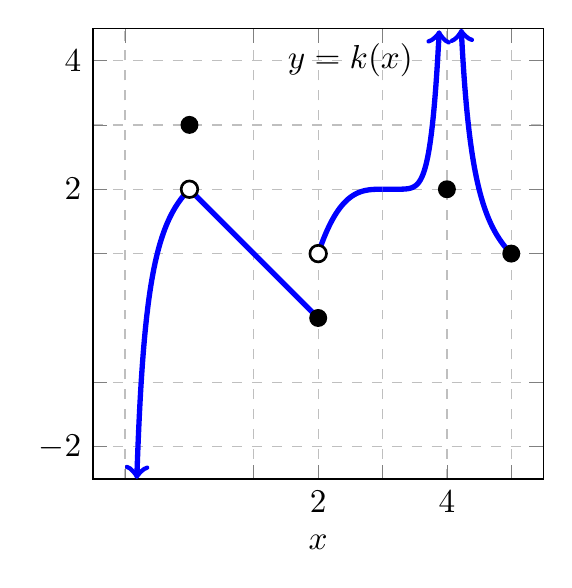
\begin{tikzpicture}[scale=1.2]
  \begin{axis}[
    xlabel={$x$},
    xtick       = {-1,1,2,3,4,5},
    xticklabels = { , ,$2$, ,$4$,},
    ytick       = {-2,-1,1,2,3,4},
    yticklabels = {$-2$, , ,$2$, ,$4$},
    samples     = 320,
    domain      = -2.5:5.5,
    restrict y to domain=-2.5:4.5,
    xmin = -1.5, xmax = 5.5,
    ymin = -2.5, ymax = 4.5,
    width = 2.5in, height = 2.5in,
    grid=both, grid style=dashed
  ]
  \node at (2.5,4) {$y=k(x)$};
  % pieces 1 & 2
  \addplot[domain=-1:0, blue, ultra thick, mark=none, <-] {3-1/(x+1)};
  \draw[blue, ultra thick] (0,2) -- (2,0);
  \filldraw[white] (0,2) circle (2.5pt);
  \draw[thick] (0,2) circle (2.5pt);
  \filldraw (0,3) circle (2.5pt);
  \filldraw (2,0) circle (2.5pt);
  % piece 3
  \addplot[domain=2:3, blue, ultra thick, mark=none] {(x-3)^3+2};
  \addplot[domain=3:4, blue, ultra thick, mark=none, ->] {6*(x-3)^7+2};
  \filldraw[white] (2,1) circle (2.5pt);
  \draw[thick] (2,1) circle (2.5pt);
  % piece 4
  \addplot[domain=4:5, blue, ultra thick, mark=none, <-] {1/(x-4)};
  %\addplot[domain=4:5, blue, ultra thick, mark=none] {-7*(x-5)^7+1};
  \filldraw (4,2) circle (2.5pt);
  \filldraw (5,1) circle (2.5pt);
\end{axis}
\end{tikzpicture}
}{
\newcommand{\spa}{.25}
\begin{enumerate}
\item[(a)] $\displaystyle\lim_{x\to0^-} f(x)=\dotfill$ \unline{.5}{\blue{$2$} }{\spa}\\
\item[(b)] $\displaystyle\lim_{x\to0^+} f(x)=\dotfill$\unline{.5}{ \blue{$2$} }{\spa}\\
\item[(c)] $\displaystyle\lim_{x\to0} f(x)=\dotfill$ \unline{.5}{ \blue{$2$} }{\spa}\\
\item[(d)] $\displaystyle\lim_{x\to2^-} f(x)=\dotfill$ \unline{.5}{ \blue{$0$} }{\spa}\\
\item[(e)] $\displaystyle\lim_{x\to2^+} f(x)=\dotfill$ \unline{.5}{ \blue{$1$} }{\spa}\\
\item[(f)] $\displaystyle\lim_{x\to2} f(x)=\dotfill$ \unline{.5}{ \blue{$DNE$} }{\spa}\\
\end{enumerate}
}{
\newcommand{\spa}{.25}
\begin{enumerate}
\item[(g)] $\displaystyle\lim_{x\to4^-} f(x)=\dotfill$ \unline{.5}{ \blue{$\infty = $ DNE} }{\spa}\\
\item[(h)] $\displaystyle\lim_{x\to4^+} f(x)=\dotfill$ \unline{.5}{ \blue{$\infty = $ DNE}}{\spa}\\
\item[(i)] $\displaystyle\lim_{x\to4} f(x)=\dotfill$ \unline{.5}{ \blue{$\infty = $ DNE} }{\spa}\\
\item[(j)] $\displaystyle\lim_{x\to-1^+} f(x)=\dotfill$ \unline{.5}{\blue{$-\infty = $ DNE}}{\spa}\\
\item[(k)] $\displaystyle\lim_{x\to1} f(x)=\dotfill$ \unline{.5}{\blue{$1$} }{\spa}\\
\end{enumerate}
}



\newpage
\paragraph*{Note:} Problems labeled as {\bf\color{blue}Extra Practice} or {\bf\color{blue} Exam Practice} should be completed on your own for you to test your comprehension of the lesson's content, with {\bf\color{blue} Exam Practice} problems corresponding to actual exam prompts from previous semesters. The particular problem below appeared on an assessment during the Spring 2024 semester and corresponds to learning target {\bf\color{RoyalBlue}L1}. 

\

Importantly, notice that exam problems are not identical to problems seen in lessons -- but still test comprehension of the very same ideas seen in lessons. {\bf You should expect to need to adjust how you prepare for this class accordingly!}

\

Please do reach out to your instructor if you need tips on how best to prepare to be successful in this class!

\

{\bf\color{blue} Exam Practice 1.}\ltrm{\bf\color{RoyalBlue}L1} Use the seven answer choices given below to respond to the prompts that follow.  Write all correct answer choices in the blanks provided. Briefly explain your answers in the spaces provided.

\

\,\hfill
        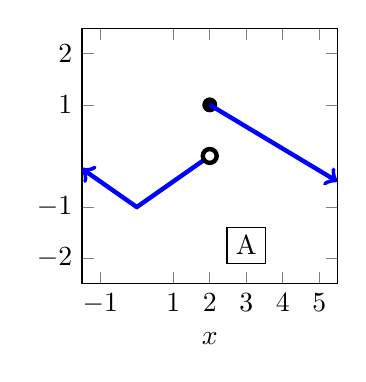
\begin{tikzpicture}[scale=1]
          \begin{axis}[
            xlabel={$x$},
            xtick       = {-1,1,2,3,4,5},
            xticklabels = {$-1$,$1$,$2$,$3$,$4$,$5$},
            ytick       = {-2,-1,1,2},
            yticklabels = {$-2$,$-1$,$1$,$2$},
            samples     = 320,
            domain      = -3:3,
            restrict y to domain=-5:5,
            xmin = -1.5, xmax = 5.5,
            ymin = -2.5, ymax = 2.5,
            width=1.9in, height=1.9in,
            %grid=both, grid style=dashed
          ]
          \node at (3,-1.75) {\fbox{A}};
          \addplot[<-,domain=-1.5:2, blue, ultra thick] {abs(x/2)-1};
          \filldraw[fill=white, ultra thick] (2,0) circle (2.5pt);
          \filldraw (2,1) circle (2.5pt);
          \draw[->, ultra thick, blue] (2,1) -- (5.5,-0.5);
        \end{axis}
        \end{tikzpicture}
\hfill
        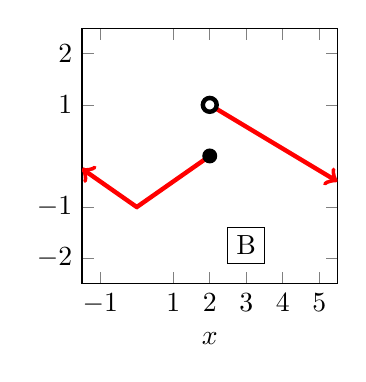
\begin{tikzpicture}[scale=1]
          \begin{axis}[
            xlabel={$x$},
            xtick       = {-1,1,2,3,4,5},
            xticklabels = {$-1$,$1$,$2$,$3$,$4$,$5$},
            ytick       = {-2,-1,1,2},
            yticklabels = {$-2$,$-1$,$1$,$2$},
            samples     = 320,
            domain      = -3:3,
            restrict y to domain=-5:5,
            xmin = -1.5, xmax = 5.5,
            ymin = -2.5, ymax = 2.5,
            width=1.9in, height=1.9in,
            %grid=both, grid style=dashed
          ]
          \node at (3,-1.75) {\fbox{B}};
          \addplot[<-,domain=-1.5:2, red, ultra thick] {abs(x/2)-1};
          \draw[->, ultra thick, red] (2,1) -- (5.5,-0.5);
          \filldraw[fill=white, ultra thick] (2,1) circle (2.5pt);
          \filldraw (2,0) circle (2.5pt);
        \end{axis}
        \end{tikzpicture}
\hfill
        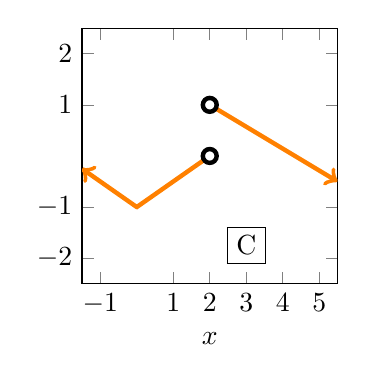
\begin{tikzpicture}[scale=1]
          \begin{axis}[
            xlabel={$x$},
            xtick       = {-1,1,2,3,4,5},
            xticklabels = {$-1$,$1$,$2$,$3$,$4$,$5$},
            ytick       = {-2,-1,1,2},
            yticklabels = {$-2$,$-1$,$1$,$2$},
            samples     = 320,
            domain      = -3:3,
            restrict y to domain=-5:5,
            xmin = -1.5, xmax = 5.5,
            ymin = -2.5, ymax = 2.5,
            width=1.9in, height=1.9in,
            %grid=both, grid style=dashed
          ]
          \node at (3,-1.75) {\fbox{C}};
          \addplot[<-,domain=-1.5:2, orange, ultra thick] {abs(x/2)-1};
          \filldraw[fill=white, ultra thick] (2,0) circle (2.5pt);
          \draw[->, ultra thick, orange] (2,1) -- (5.5,-0.5);
          \filldraw[fill=white, ultra thick] (2,1) circle (2.5pt);
        \end{axis}
        \end{tikzpicture}
\hfill\,\\
        
\,\hfill
        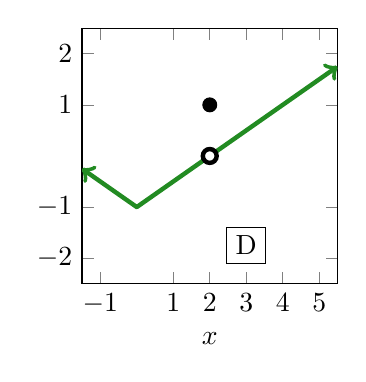
\begin{tikzpicture}[scale=1]
          \begin{axis}[
            xlabel={$x$},
            xtick       = {-1,1,2,3,4,5},
            xticklabels = {$-1$,$1$,$2$,$3$,$4$,$5$},
            ytick       = {-2,-1,1,2},
            yticklabels = {$-2$,$-1$,$1$,$2$},
            samples     = 320,
            domain      = -3:3,
            restrict y to domain=-5:5,
            xmin = -1.5, xmax = 5.5,
            ymin = -2.5, ymax = 2.5,
            width=1.9in, height=1.9in,
            %grid=both, grid style=dashed
          ]
          \node at (3,-1.75) {\fbox{D}};
          \addplot[<->,domain=-1.5:5.5, ForestGreen, ultra thick] {abs(x/2)-1};
          \filldraw[fill=white, ultra thick] (2,0) circle (2.5pt);
          \filldraw (2,1) circle (2.5pt);
        \end{axis}
        \end{tikzpicture}
\hfill
        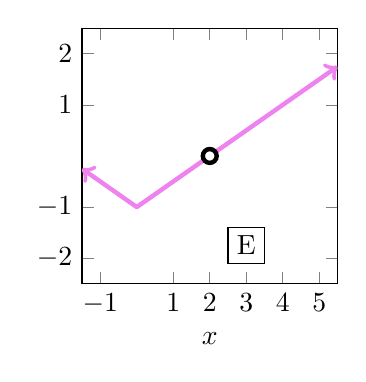
\begin{tikzpicture}[scale=1]
          \begin{axis}[
            xlabel={$x$},
            xtick       = {-1,1,2,3,4,5},
            xticklabels = {$-1$,$1$,$2$,$3$,$4$,$5$},
            ytick       = {-2,-1,1,2},
            yticklabels = {$-2$,$-1$,$1$,$2$},
            samples     = 320,
            domain      = -3:3,
            restrict y to domain=-5:5,
            xmin = -1.5, xmax = 5.5,
            ymin = -2.5, ymax = 2.5,
            width=1.9in, height=1.9in,
            %grid=both, grid style=dashed
          ]
          \node at (3,-1.75) {\fbox{E}};
          \addplot[<->,domain=-1.5:5.5, Violet, ultra thick] {abs(x/2)-1};
          \filldraw[fill=white, ultra thick] (2,0) circle (2.5pt);
          %\filldraw (2,1) circle (2.5pt);
        \end{axis}
        \end{tikzpicture}
\hfill
        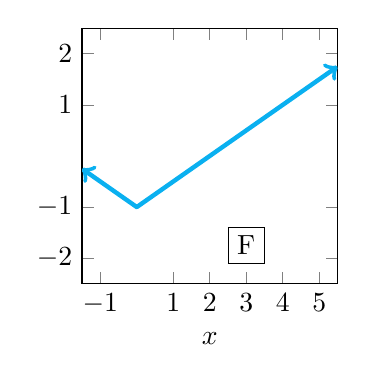
\begin{tikzpicture}[scale=1]
          \begin{axis}[
            xlabel={$x$},
            xtick       = {-1,1,2,3,4,5},
            xticklabels = {$-1$,$1$,$2$,$3$,$4$,$5$},
            ytick       = {-2,-1,1,2},
            yticklabels = {$-2$,$-1$,$1$,$2$},
            samples     = 320,
            domain      = -3:3,
            restrict y to domain=-5:5,
            xmin = -1.5, xmax = 5.5,
            ymin = -2.5, ymax = 2.5,
            width=1.9in, height=1.9in,
            %grid=both, grid style=dashed
          ]
          \node at (3,-1.75) {\fbox{F}};
          \addplot[<->,domain=-1.5:5.5, ProcessBlue, ultra thick] {abs(x/2)-1};
          %\filldraw[fill=white, ultra thick] (2,0) circle (2.5pt);
          %\filldraw (2,1) circle (2.5pt);
        \end{axis}
        \end{tikzpicture}
\hfill\,\\

\,\hfill \fbox{G} none of the other answers \hfill\,\\

\

%\,\hfill {\noindent } \hfill\,

\

\begin{enumerate}
%\item[(a)] Which of the answer choices could be the graph of a function $f$ for which $f(2)=0$? \hrulefill

%\vfill

\item[(a)] Which of the answer choices could be the graph of a function $g$ for which $\displaystyle\lim_{x\to2} g(x)$ DNE? \hfill \unline{.8}{\blue{A,B,C}}

\sol{
In all three cases, $\ds \lim_{x\to 2^-} g(x)\neq \lim_{x\to 2^+} g(x) \Rightarrow \lim_{x\to 2} g(x)= DNE$
}

\item[(b)] Which of the answer choices could be the graph of a function $h$ for which $\displaystyle\lim_{x\to2} h(x)=1$? \hfill\unline{.8}{ \blue{G}}

\sol{
In all cases, $\lim_{x\to 2^-} h(x)=0 \neq 1$.  Since limit from left side is  $0$, none will result in $\ds \lim_{x\to 2}h(x)=1$ and thus the best answer is G.
}

\item[(c)] Which of the answer choices could be the graph of a function $k$ for which $\displaystyle\lim_{x\to2} k(x)=0$?\hfill \unline{.8}{ \blue{D, E, F}}

\sol{
For D, E, and F, $\ds \lim_{x\to 2^-}k(x)=0= \lim_{x\to 2^+}k(x)$. Since limit from left and right are same, we can conclude $\ds \lim_{x\to 2}k(x)=0$. This is not true for A, B, C.
}

\end{enumerate}

\end{document}
